%%%%%%%%%%%%%%%%%%%%%%%%%%%%%%%%%%%%%%%%%%%%%%%%%%%%%%%%%%%%%%%%
%% DOCUMENT %%
%%%%%%%%%%%%%%%%%%%%%%%%%%%%%%%%%%%%%%%%%%%%%%%%%%%%%%%%%%%%%%%%

% fleqn = left align equations
\documentclass[fleqn,a4paper,12pt]{book}

%%%%%%%%%%%%%%%%%%%%%%%%%%%%%%%%%%%%%%%%%%%%%%%%%%%%%%%%%%%%%%%%
%% Packages %%
%%%%%%%%%%%%%%%%%%%%%%%%%%%%%%%%%%%%%%%%%%%%%%%%%%%%%%%%%%%%%%%%

	% Page Layout
	\usepackage[top=2.54cm, bottom=2.54cm, left=2.54cm, right=2.54cm]{geometry} % margins
	
	
	% Encodings
	\usepackage[latin1]{inputenc} 	% Source text encoding
	\usepackage[T1]{fontenc}	  	% Output glyphs encoding
	\usepackage[english]{babel}	  	% Add unicode characters
	\usepackage{textcomp} 		  	% Add antoher set of characters
	%\usepackage[cyr]{aeguill}    	% hyphenated symbols
	
    % Math
    \usepackage{amsmath}			% Math package
    \usepackage{amsfonts}			% Supplementary symbols
    \usepackage[amsmath]{ntheorem}  % Theorem layouts
    \usepackage{stmaryrd}           % special symbols for natural sets

	% Graphics
	\usepackage{graphicx}			% Graph package
	\DeclareGraphicsExtensions{.pdf,.png,.PNG,.jpg,.jpeg} 
	\graphicspath{ {./images/} }    % look into images/ for images
    
    % Captions
    \usepackage[justification=centering]{caption} % long-centered captions
    \usepackage{subcaption}			% captions for subfloat
	
	% PDF
	\usepackage{pdfpages} 			% insert pdf as images
	
	% Citations
	\usepackage[round]{natbib} 		% author-date style cites
	
	% Table and Arrays
	% \usepackage{exceltex} 		% insert excels tables in tex (macro)
	\usepackage{booktabs} 			% Pretty tables
	\usepackage{array}				% for fixed-width columns and alignments 
    
    % Source Code
    \usepackage{listings}			% Insert programming langage code
    
	% URL
    \usepackage{hyperref}			% handle url and hyperlinks
    %! This package must always be included last (it's a linker operation). !%
    
%%%%%%%%%%%%%%%%%%%%%%%%%%%%%%%%%%%%%%%%%%%%%%%%%%%%%%%%%%%%%%%%
%%  Styles
%%%%%%%%%%%%%%%%%%%%%%%%%%%%%%%%%%%%%%%%%%%%%%%%%%%%%%%%%%%%%%%%

% Code Printing configuration
\lstset{
    language=Python,
    basicstyle=\small\sffamily,
    numbers=left,
    numberstyle=\tiny,
}

% Definition and Theorem layouts
\newtheorem{mydef}{Definition}

\theoremstyle{break}                  
\newtheorem{mytheorem}{Theorem}

%%%%%%%%%%%%%%%%%%%%%%%%%%%%%%%%%%%%%%%%%%%%%%%%%%%%%%%%%%%%%%%%
%% Commands
%%%%%%%%%%%%%%%%%%%%%%%%%%%%%%%%%%%%%%%%%%%%%%%%%%%%%%%%%%%%%%%%

%HRule : make a horizontal line
\newcommand{\HRule}{\rule{0.95\textwidth}{0.5mm}}

%noi = noindent
%\newcommand{\noi}{\noindent}

%alias for XOR operator.
\newcommand{\xor}{\oplus}


%%%%%%%%%%%%%%%%%%%%%%%%%%%%%%%%%%%%%%%%%%%%%%%%%%%%%%%%%%%%%%%%
%% Title Page
%%%%%%%%%%%%%%%%%%%%%%%%%%%%%%%%%%%%%%%%%%%%%%%%%%%%%%%%%%%%%%%%
\title{Cryptography I - Notes \vfill}
\author{lucasg}


% Remove every indentation (personnal style). 
\setlength\parindent{0pt}
%%%%%%%%%%%%%%%%%%%%%%%%%%%%%%%%%%%%%%%%%%%%%%%%%%%%%%%%%%%%%%%%
%% BODY
%%%%%%%%%%%%%%%%%%%%%%%%%%%%%%%%%%%%%%%%%%%%%%%%%%%%%%%%%%%%%%%%
\begin{document}

\maketitle

%%%%%%%%%%%%%%
%% Abstract
\vspace*{6cm}
\hfill
\begin{minipage}[c]{0.8\linewidth}
\begin{Large}
%\begin{flushleft}

These notes are based upon the free Coursera Course called "Cryptography I", teached by Dan Boneh from Standford, as well as information gathered from Wikipedia.\\
First, it's  a personal project from an amateur in the domain : it is not exempt from errors and imprecisions (as well as grammar/typos since I am not an native English speaker).\\
Second, the way the document is structured does not make it easy for a complete beginner to understand cryptography : I assume readers have to be somewhat proficient in mathematics and computer science to understand big-O notations, P/NP problems, and basic algebra (sets, group theory, etc.). \\

This document was written using ShareLatex, a powerful web-based editor, and shared using Github (lucasg/crypto-report1).

%\end{flushleft}
\end{Large}
\end{minipage}


%%%%%%%%%%%%%%
%% TOC
\tableofcontents

%%%%%%%%%%%%%%
%% Chapters


\chapter{Introduction}



A cipher consist of en encoder and a decoder. The algorithm behind the encoder and the decoder has to be public in order to ensure the integrity and the robustness of the cipher. The ciphers are typically  open source projects, reviewed by security experts.  \\

\subsection{Definitions}

\begin{flalign*}
\emph{Encoder : }  &E : KxM \mapsto C  \\
\emph{Decoder : }  &D : KxC \mapsto M  \\ 
\emph{Equality : } &D(k, E(k,m) ) = m  
\end{flalign*}

E is often randomized whereas D is always deterministic. A cipher consist of the encoder and decoder : cipher $=$ $(E,D)$.



\begin{figure}[ht!]
	\centering
		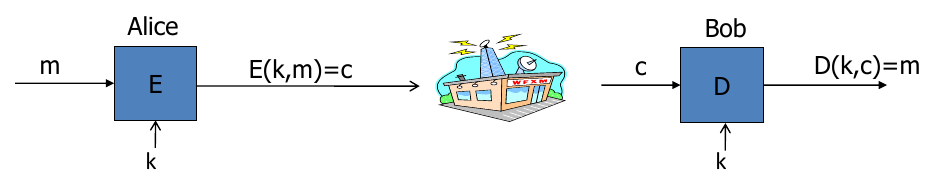
\includegraphics[width=0.7\textwidth]{images/tata}
	\caption{Cipher}
	\label{fig:Cipher}
\end{figure}

A common mistake is to think that an ad-hoc crypto algorithm with closed source is safer than open source standards : the big problem with closed source algorithms is that, when they are breached, the user does not know.\\


Uses of crypto : 
\begin{itemize}
		\item Secure communication : private conversations without eavesdropping 
		\item Digital signatures : secure identification (no tampering)
		\item Anonymous communication : secure and private communication without any of the participants know the identity of the others  
		\item Anonymous computation : outsourcing computation without giving the purpose of the calculus to the contractor (e.g. Amazon w3s)\\
\end{itemize}

\subsection{Trusted authority}

One way to ensure confidentiality is to outsource the task to a third party which has credibility and trust, like when we give our last will to a exterior person which does not have any involvement with the family(typically a \emph{notaire}).

However, the trusted authority solution - like any centralized mecanism -  creates a single point of failure, so the trusted authority might not be always a good solution. \\

\emph{Theorem} : Any computation done by trusted authority can be done without it.\\


\subsection{ Zero proof of knowledge }

\textit{Aim of cryptography} : prove that, under a certain threat vector, forge the signature comes to solve a NP-problem. \\

The definition of a NP-problem is that it is computationally "hard" to solve (nondeterministic polynomial time), but easy to verify a solution (called signature).

A zero-knowledge proof is a signature the user present to the server, which will answer true or false based on the signature's validity. Under zero-knowledge hypothesis, the user does not learn anything more than the validity of the signature.

\subsection{History of ciphers}

Cryptology is an ancient matter : all sorts of encoding scheme has been invented throughout History. \\


\emph{Definition :} $E(k,m)$ is the encryption of message $m$ using key $k$. (the key always first ) \\
\emph{Definition :} $D(k,c)$ is the decryption of ciphertext $c$ using key $k$. (the key always first ) 

\subsubsection{Substitution cipher }
The substitution cipher ( also called Caesar cipher in its weak form ) is a simple encoder, yet relatively effective : the key $K$ is a bijective map between two alphabets. For example, $A$ becomes $C$, $B$ becomes $O$, etc.\\

\begin{table}[ht!]
    \centering
    \scalebox{0.9}{
		\begin{tabular}{|c|c|c|c|c|c|c|c|c|c|c|c|c|c|c|c|c|c|c|c|c|c|c|c|c|c|c|}
			\hline
$input$&a&b&c&d&e&f&g&h&i&j&k&l&m&n&o&p&q&r&s&t&u&v&w&x&y&z \\
$output$&c&o&a&h&l&z&m&v&n&e&b&q&s&j&u&k&w&r&p&g&t&i&d&x&f&y \\
            \hline
		\end{tabular}
    }
	\caption{Substituion table}
	\label{tab:SubstitionTable}
\end{table}

Example of a encryption : 
\begin{alignat*}{3}
    &\text{plaintext}   & : & \text{ several flamethrowing sharks}&  \\
    & \downarrow        & : &   \downarrow & \\
    &\text{cyphertex}   & : & \text{ plilrcq   zqcslgvrudlr pvcrbp}&  \\ 
\end{alignat*}


The encryption is simply the substitution of every letter in the message $m$ by its counterpart in the map $K$.\\
The substitution cipher is however breakable just by looking at ciphertexts. The study of the letters' frequencies in the ciphertexts can give huge informations on the map $K$. In English, the letter "$e$" is the most used so, by looking which letter is the most used in the ciphertexts, we can give a pretty good guess of the subsitution of "$e$".\\

\begin{figure}[ht!]
    \centering
		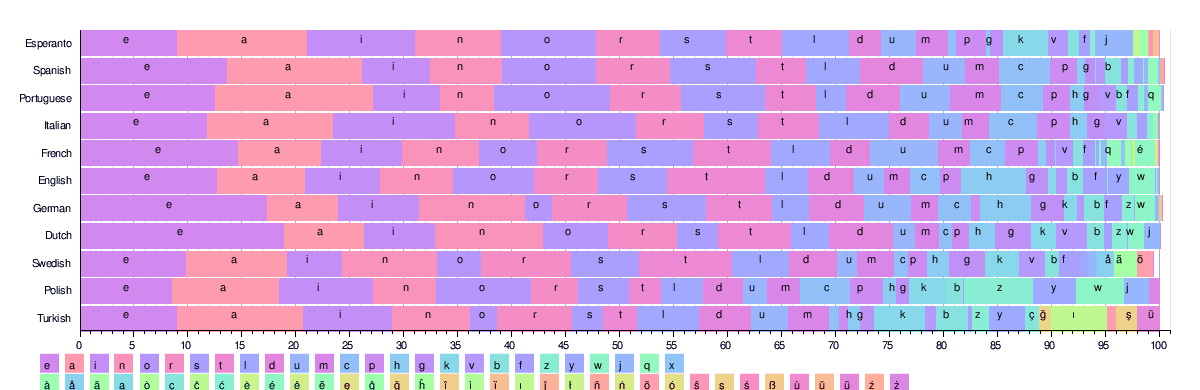
\includegraphics[width=\textwidth]{images/letter_frequency}
	\caption{Letter frequencies in several languages. It is fairly easy to guess the message's language just by looking at letter's repartition. \\ source : Wikipedia}
	\label{fig:LetterFrequency}
\end{figure}

The Caesar cipher is a simpler (and weaker) version of the substitution cipher : every character in the alphabet is offsetted by a constant value (modulo the alphabet's length). For example $A$ become $C$, $B$ become $D$, and so one... In this form, the key is not a map anymore, but only a constant integer,which is far smaller. 

\newpage
\begin{minipage}[c]{\linewidth}
    \lstinputlisting[
        language=Python,
        label= SubstitutionCode,
        caption=Substitution Code (in Python 2.7)
        ]{code/substitution.py}
\end{minipage}
\vfill


\subsubsection{ Vigenere cipher }

The  Vigenere cipher is built from the substitution code. The cipher use a work as key : every character will be used as a Caesar cipher encryption scheme. 
Example of a encryption : 
\begin{alignat*}{3}
    &\text{plaintext}   & : & \text{flamethrower}&  \\
    &\text{key}         & : & \text{vigenerecode}&  \\
    &\text{cyphertex}   & : & \text{ztgqrayvqkhv}&  \\ 
\end{alignat*}

If yhe encryption is based on a sum of letter position in the alphabet modulo the alphabet's length, the decryption is as simple since it's a difference: 

Example of a decryption : 
\begin{alignat*}{3}
    &\text{plaintext}   & : & \text{ztgqrayvqkhv}&  \\
    %&\text{plaintext} &:& \text{------------}&  \\
    &\text{key}         & : & \text{vigenerecode}&  \\
    %&\text{plaintext} &:& \text{____________}&  \\
    &\text{cyphertex}   & : & \text{flamethrower}&  \\ 
\end{alignat*}

\begin{figure}[ht!]
    \centering
        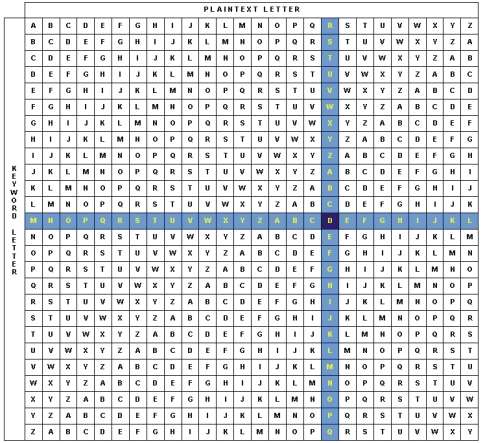
\includegraphics[width=0.7\textwidth]{images/vigenere}
	\caption{Vigenere \emph{tabula recta} for handmade encryption\\ source : illuminations.nctm.org}
	\label{fig:LetterFrequency}
\end{figure}

The Vigenere code is a fairly simple encryption scheme yet it were quite powerful (before the invention of automatic computation) since the encryption/decryption is a time-linear operation (table lookups) whereas the brute-force attack involve time-polynomial operations (multiple tables creation and lookups). It is still fairly easily breakable if the key's length is known to the attacker because it revert the cipher to a substitution one. Morevover, there are several methods which estimate the key's length based on frequency analysis (the vigenere cipher does mask all letter frequency patterns).\\





On a side note, if the key is smaller than the encoding message, they key is repeated and padded to match the message's length:
\begin{alignat*}{3}
    &\text{plaintext}   & : & \text{several flamethrowing sharks}&  \\
    %&\text{plaintext} &:& \text{+++++++ +++++++++++++ ++++++}&  \\
    &\text{plaintext}   & : & \text{smallsm allsmallsmall smalls}&  \\
    %&\text{plaintext} &:& \text{____________}&  \\ 
    &\text{cyphertex}   & : & \text{flamethrower}&  \\ 
\end{alignat*}


\subsubsection{Enigma}

The enigma machine is a device built by a German company around 1920 and consist of rotating substitution ciphers : 

\begin{figure}[ht!]
        \centering
        \begin{subfigure}[b]{0.4\textwidth}
                \centering
                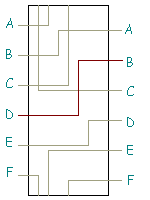
\includegraphics{images/enigma_rotor1}
                \caption{A is mapped to B}
                \label{fig:enigma_rotor1}
        \end{subfigure}
        \begin{subfigure}[b]{0.4\textwidth}
                \centering
                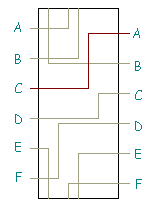
\includegraphics{images/enigma_rotor2}
                \caption{A is now mapped to C}
                \label{fig:enigma_rotor2}
        \end{subfigure}
        \caption{Enigma rotor : the rotor rotate by a increment for every new input, which lead to a different substitution table. \\ Source : www.bibmath.net }\label{fig:enigma_rotors}
\end{figure}

In order to strenghten the protocol, a typical Enigma machine use 3 rotors and a reflector\footnote{There is also a plugboard, which swap at most two pairs of letters.}. The reflector is a fixed rotor which acts as a mirror (it 's a simple substitution cipher) and each rotor is incremented by a special transition from the rotor on the left (apart from the most left one, which is incremented at each new input). In this configuration, the rotors' configurations act as public keys while the rotors' initial position as well as the rotors' order is the private one. The rotors can be sold or stolen without revealing anything about the encryption (apart from degenerate rotor configurations). The machine being symetrical, the cipher is symetric too : using the same private key, typing the ciphertext into the machine will print the plaintext message\footnote{Mathematical proof of the Enigma's symmetrical property can be found here : ??? .}.


\begin{figure}[ht!]
    \centering
        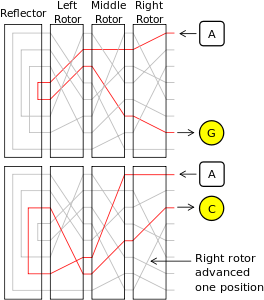
\includegraphics[width=0.7\textwidth]{images/Enigma_3rotors}
    \caption{ Enigma machine with 3 rotors and a reflector.\\ source : Wikipedia}
	\label{fig:enigma_3rotors}
\end{figure}

The enigma machines were largerly used during World War II by the German Army as a crypto-system. The breaking of Enigma di occupy a lot of mathematicians and logicians at that time, and bring numerous breakthroughs in cryptology. Finally, Alan Turing \footnote{also known as the most badass computer scientist of the 20th century} did crack the cipher using "crib" techniques : by analysing ciphertexts and some partial plaintexts (such as headers, known contents,...), it was possible to deduce the inner structure of the machine, and creating an automatic decypher called \emph{Bombe}.







\chapter{Theory}

\section{Definitions}

\subsection{Symmetric/Asymmetric Ciphers}

\begin{mydef}
\begin{minipage}[t]{0.8\textwidth}
    A cipher is symmetric if the encryption $E$ and the decryption $D$ use the same key $k$.
\end{minipage}
\end{mydef}

\begin{mydef}
\begin{minipage}[t]{0.8\textwidth}
    A cipher is asymmetric if the encryption $E$ and the decryption $D$ do not the same key. The encryption key is often called "public key" and the decryption one "private key".
\end{minipage}
\end{mydef}

The symmetric-key encryption is the oldest class of cryptography process. The major flaw of symmetric ciphers is the obligation for both parties (sender and receiver) to share the secret (the key). Nowadays, it is recommended to use non-symmetric encryption (also known as public-key encryption).

%\subsection{Computationally equivalence}
%Definition : two distributions $P_1$ and $P_2$ are computationally equivalent if , %for every "efficient" polynomial statistical test A, \\

%$ | Pr[A(X) == 1  - Pr[A(X) == 1] |  $ \\
%$   X <- P_1      X <- P_2              $ \\
%X chosen uniformly dans les distributions.

%\section{Probability Remainder}

\section{ Pseudo-Random Generation }

\subsection{Statistical test for Randomness}

Pseudorandomness is the property of a function to appear random, while being completely deterministic. In cryptography, the pseudorandomness property for a bit generator is an important one : the security is often built upon it since the attacker cannot predict the output. That's why a lot of different statistical test were conceived to separate true pseudorandom generators from broken ones (bit-frequency, chi-square Test, arithmetic mean, ...).

\begin{mydef}
A statistical test is an algorithm which, given a generator, ouptut 0 or 1 based on the stream of numbers generated, 1 being random and 0 deterministic.
\end{mydef}

\paragraph{Advantage \\}
\label{sec:advantage}

Let F an oracle\footnote{an oracle is a computational black box} which we want to study and G a perfect one implementing true randomness. The advantage $Adv$ over F, using the statistical test A, is: 
\begin{mydef}
$Adv_{F} [A,G] = | Pr[A(G(k)) == 1  - Pr[A(G(r)) == 1] | \in  [0,1] $
\end{mydef}

An advantage "close to one"\footnote{it really depends on the security margin} is considered to break the pseudorandom function, because the test A can distinguish pseudo-randomness from true randomness.


\subsection{Pseudo-Random Functions   (PRF)}

A pseudo-random function is a fairly easily computable function (~polynomial) which simulate randomness while being completely deterministic.

\paragraph{Definition \\}
Let $F$ a function from $KxD$ to $R$ which maps a two set (the domain $M$ and the range $R$) using a key parameter from $K$ : the function F is a PRF if no efficient adversary with significant advantage can distinguish F from a random oracle. Pseudo-random functions are vital tools in the construction of cryptographic primitives.

\paragraph{Secure PRF \\}
\label{sec:IND-Game-PRF}

A pseudorandom function is secure if an attacker cannot solve the following game with a significant advantage :

\begin{figure}[h!]
	\centering
		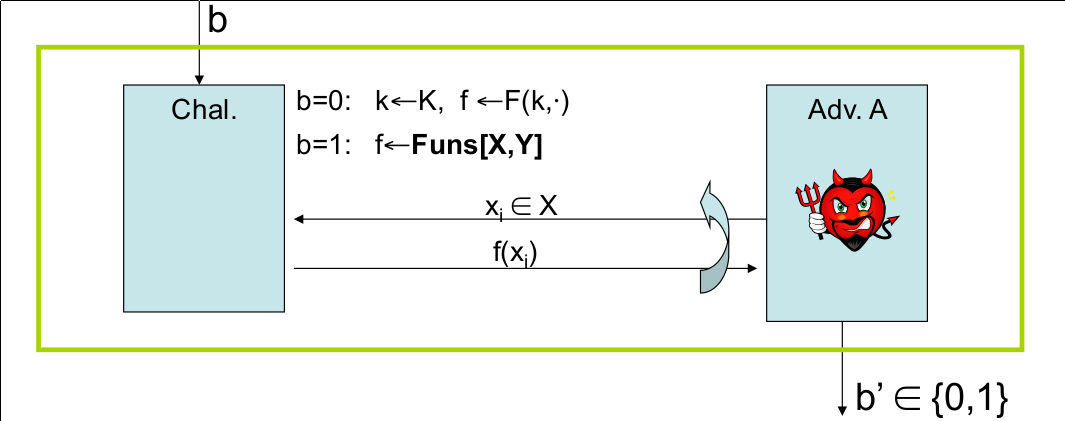
\includegraphics[width=0.7\textwidth]{secure-PRF.png}
	\caption{indistinguishability game for PRF}
	\label{fig:Cipher}
\end{figure}

Let b a binary value and $F: X\times K \rightarrow Y$  a PRF from $X$ to $Y$. If $b$ is null, the oracle will chose a random key $k\in K$, otherwise it will choose a complete random function $f:X->Y$. Then the adversary A submit one or several value(s) $x_i \in X$ and get the result $y_i \in Y$, from either the pseudo-random function or the randomly chosen one (according to the value of $b$). The attacker must find which function the oracle used, and if it find it with an advantage(see \ref{sec:advantage}), the PRF is considered insecure.


\subsection{Pseudo-Random Permutation   (PRP)}


\paragraph{Definition \\}

A PRP differs from a PRF in the way that the domain $D$ and the range $R$ are the same. Since the function map the two same sets, we can deduce that $E(k,.)$ ( k is fixed) is bijective : it is a permutation then.
A major propriety of the PRP (comparatively to the PRF) is that the PRP can be inverted, thus improving the decoding speed.\footnote{Another useful property is that permutation can be chained or cascaded since they all have the same working domain.}

\paragraph{Secure PRP \\}


\begin{figure}[ht!]
	\centering
		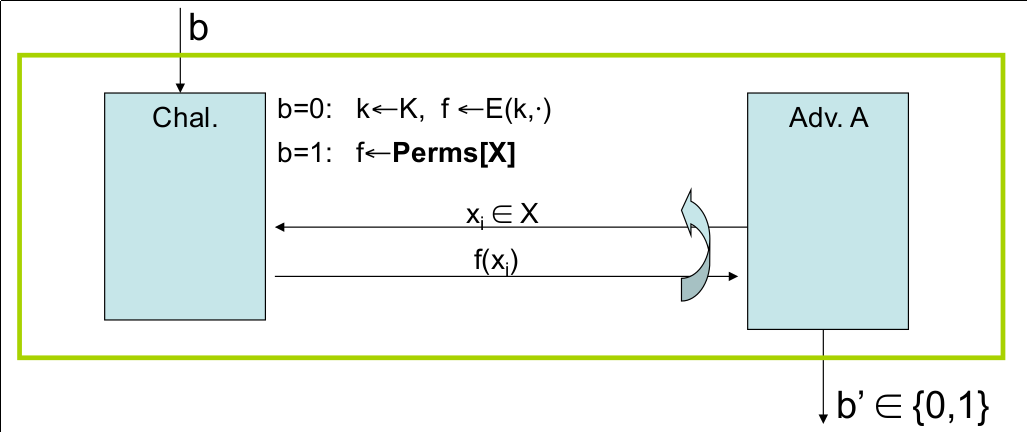
\includegraphics[width=0.7\textwidth]{secure-PRP.png}
	\caption{indistinguishability game for PRP}
	\label{fig:Cipher}
\end{figure}

The challenge for PRP is not much different from the one on PRF : see \ref{sec:IND-Game-PRF}.

\subsection{Pseudo Random Generator     (PRG)} 


\paragraph{Definition \\}

A pseudo random generator (PRG) is a deterministic bit generator with the property of  unpredictability :
\begin{mydef}
$ G : \llbracket  0,1 \rrbracket ^s -> \llbracket  0,1 \rrbracket ^n $  with  $n>>s$. \\ $S = \llbracket  0,1 \rrbracket ^s$ is often called "the seed" and is randomly chosen. 
\end{mydef}

Stream ciphers are easily built from PRG : $c = m \oplus G(k) $  (one time pad with pseudo-random generator )


\paragraph{Secure PRG \\}
A PRG is secure if, for all "efficient" statistical test A, $Adv(A,G)$ is negligible.

On a side note, we don't know all the existing efficient statistical tests so we can't prove that PRG is secure, we can only prove we didn't found an efficient test which break it.


\section{Confidentiality}
\subsection{Perfect Secrecy}

\begin{mytheorem}[Shannon perfect secrecy]
    $\forall m_1,m_2$ such as $len(m_1) = len(m_2)$, 
    $Pr[E(k,m_1) = c] = Pr[E(k,m_2) = c]$  \flushright (k uniform in K)
\end{mytheorem}

In layman terms, perfect secrecy means that, given two messages and the ciphertext of one of the two plaintext messages, the attacker cannot know from which message the ciphertext has been created (equal probability). A corollary is, under perfect secrecy conditions, the key space $K$ cardinality must be equal or larger than the ciphertext space $C$ cardinality, which has to be equal or larger than the message space $M$ cardinality :
\begin{mytheorem}[Shannon perfect secrecy corollary]
    $ |M| \leq |C| \leq |K| $. 
\end{mytheorem}


\subsection{Semantic Security}

The semantic security is a weaker form of Shannon's perfect secrecy (which is not usable in reality) : the distributions $P_1 = Pr[E(k,m_1) = c , k<- K]$ and $P_2$ does not have to be equal, just computationally equivalent.

\paragraph{Challenge}
The semantic security is often defined using a "challenge" : an experiment of though where and adversary has to find an important information given a certain protocol and certain rights. The challenge is the following one :

\begin{figure}[ht!]
	\centering
		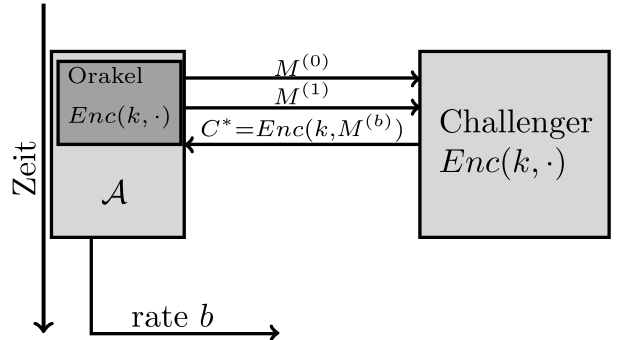
\includegraphics[width=0.7\textwidth]{IND-CPA-Game.png}
	\caption{Semantic security challenge}
	\label{fig:SemanticSecurityChallenge}
\end{figure}

The challenger (the "defender") choose a fixed-key and a variable $b$ randomly from two values ( 0 and 1 to be simple). The attacker then will send the challenger $2*n$ messages (plain or encrypted) and the challenger only process half of them (given the value b) and send the result back to the attacker.\\
The attacker has to estimate the value $b$ chosen : if the attacker can guess the value of b with a significant advantage, the encryption cipher is considered insecure. Otherwise, it has semantic security against the corresponding attack channel.

\paragraph{Semantic Security against Chosen Plaintext Attack (CPA)\\}

In this configuration, the attacker can choose which plaintext message(s) to send to the challenger, and has the result of the encryption of half of them. 

\begin{mytheorem}[Semantic Security under CPA]
    $E$ is semantically secure  under chosen plaintext attack if, for all adversary A, $Adv_{CPA}[A,E] = Pr()$ is negligible.
\end{mytheorem}

\paragraph{Semantic Security against Chosen Ciphertext (Adaptive) Attack ($CCA-1$/$CCA-2$)\\}

In this configuration, the attacker can choose which ciphertext message(s) to send to the challenger, and has the result of the decryption of half of them. Under $CCA-2$ he can also makes incremental changes to the ciphertext sent given the output the previous decryption, enabling linear and differential attacks. \\
The $CCA$ assumption allow the attacker a wide range of access to information : the protocols which are secure against $CCA$ are extremely useful since they can withstand a great variety of attacks \footnote{of course, there still are side-channel attacks.}.

\section{Integrity}
\subsection{Secure MAC}


%\section{Number Theory}

\chapter{Attack Vectors}


\section{Exhaustive Search Attack}
    The Exhaustive search attack, or brute-force attack, is to try every key possible until we retrieve the plaintext message. Although very crude and somewhat inefficient, some ciphers are unfortunately weak against it: the DES is one of them.
    
\paragraph{Definition :}
Given $(m_i,c_i)$ in $\llbracket 1,N \rrbracket$(with N a small integer), find key k.

\paragraph{DES Challenge (by RSA)\\}
The aim of the DES Challenge is to find the secret key given three messages and their encryption. It was organized by the RSA company, to demonstrate the vulnerability of DES (the good ol' naming and shaming technique ).

\begin{description}
\item[1997 : ] 3 months using Internet-distributed computation ("cloud" computing)
\item[1998 : ] 3 days using EFF\footnote{Electronic Frontier Foundation : a NGO focusing on net freedom}'s deep crack machine.
\item[1999 : ] 22 hours
\item[2006 : ] 7 days using 10k\$'s FPGAs.
\end{description}

\paragraph{Prevention}
You only way to prevent a cipher from ESA is to augment the key size until no existing computation power can break the cipher in a reasonable time (like centuries).

\section{Cryptographic attacks}
The cryptographic attacks are the generic attack types used when talking about theoretical security (like semantic security).

\paragraph{Known Plaintext  \\} The attacker has in his possession a plaintext message and its corresponding encryption.

\paragraph{Cyphertext Only  \\} The attacker does not know the plaintext message and has to find out (see Cesar cipher's breaking technique).

\paragraph{Chosen Plaintext/Cyphertext \\} 
The attacker can respectively encrypt/decrypt any plaintext/cyphertext message and study the result. It is the most common paradigm when studying public key cryptography (the attacker know the public key and can encrypt any message of his will).

\paragraph{Adaptative Plaintext/Cyphertext \\} 
The attacker can iterate the encryption/decryption based on the previous result (used for linear and differential attacks).

\section{Side-channel attacks}
Side-channel attacks are "real-world" attacks, i.e. they don't rely on theoretical cryptographic knowledge but rather the implementation of ciphers. \footnote{ They are considered "inelegant", but the result is what matters, is it not ?}

\paragraph{Attack on the implementation \\}
Some perfectly secure ciphers can be compromised if they are implemented in the wrong way : buffer overflows on user input, stack overflows, information leaking, insufficient entropy, ...   

\paragraph{Hardware Attacks \\}
Another way to look at implementation is to consider the hardware : the analysis of the time and power required to encode/decode messages (using oscilloscopes and multimeter) can reveal important informations about the cipher used.

\paragraph{Fault Attacks \\}
This attack is a follow up of the previous ones : by using laser to provoke run-time segfault (by twiddling the RAM bits), the attacker's aim is to create computing errors which can reveal informations about the key.

\section{Meet in the middle attacks}

\paragraph{Definition\\}
The MITM attacks is a generic cryptoanalysis used originally to break n-rounds block ciphers. Given the ability to encrypt and decrypt any data, the attacker will try to find the encryption of a certain plaintext which match the decryption of another certain cyphertext. In others words, the encryption and decryption algorithm does each one half of the work and "meet".

\begin{mydef}[Meet in the middle Attack :]
b \newline
\begin{minipage}[t]{0.8\textwidth}
	Given (E,D) encryption/decryption system, \\
    Find (m,c) such that : E(m) == D(c).
\end{minipage}
\end{mydef}

\paragraph{Example}

A famous example which validate the theory of "more rounds equal better security" is the double-DES : once demonstrated that DES is insecure, they tried to update the standard without changing everything by simply cascading a DES into another one, using two separate keys. However, 2-DES is badly vulnerable from MITM attacks.

\begin{mydef}[Challenge :]
b \newline
\begin{minipage}[t]{0.9\textwidth}
	Given (m,c), find $k = (k_1,k_2)$ such that $E(k_1,E(k_2,m)) == c$
\end{minipage}
\end{mydef}

Since $k_1$ and $k_2$ are independent keys, we have : $E(k_2,m) = x = D(k_1,m) $ . Breaking a $2-DES$ cipher is close to break DES, just twice longer. That's why $2-DES$ was never used and standard chosen is $3-DES$.

\section{Linear and Differential Attacks}

\subsection{Linear Attacks}
\subsection{Differential Attacks}


\section{Quantum attacks}

Quantum attacks are based on quantum computing. Unlike classical computers, quantum computers take advantage of quantum state superposition and entanglement to speed up solving time of equations, especially when combinatory calculus are present.

\paragraph{ Generic Search Problem}

\begin{mydef}
\begin{minipage}[t]{0.8\textwidth}
    Let $f : X \rightarrow {0,1}$ a generic oracle, \\
  	Generic Search Problem : find $x \in X$ such as $ f(x) == true $.
\end{minipage}
\end{mydef}

On classical computer, the best generic solver is linear ( $O(|X|)$ ) whereas on a quantum computer, it's root-squared ( $O(|X|^{\frac{1}{2}})$).


\paragraph{ Consequences } 
The practical consequence of quantum computing over cryptography is to halve the key space : a way to prevent ciphers from quantum attacks is to double the key space ( a 1024-key RSA cipher is as strong against quantum computers as a 512-key RSA cipher against classical computers).


\section{Collision attacks}

When talking about collision resistance, it is important to speak about the Birthday Paradox which stipulates that there are way more random collisions than you would guess.

\subsection{Generic Birthday attacks}

The Birthday Paradox rest upon the following question : given a random group of people, what's the odds of having at least two persons with the same birthday ? The question is equivalent of estimating the probability of a collision from the output of a bounded random number generator.\\

Intuitively, we would think that the odds grow linearly with the group's size whereas, in reality, the odds grow way faster : when the group has 23 person, there is a 50\% chance of a collision ! The paradox lies here : you only need of tenth of sample from the random pool to have a fairly high chance of collision, which is not intuitive (we would rather think of needing half of the pool - more or less 180 persons -  to have a 50\% chance).

\begin{figure}[ht!]
    \centering
   	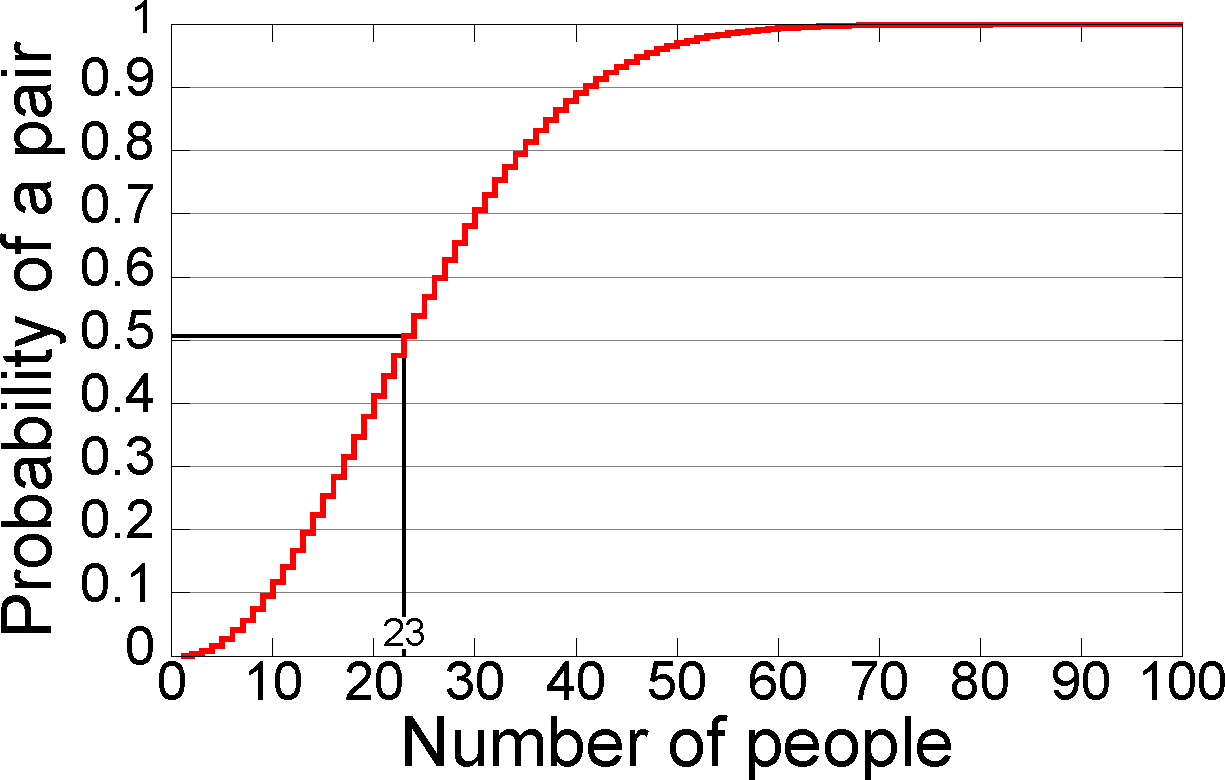
\includegraphics[width=\textwidth]{images/Birthday_Paradox.pdf}
	\caption{Probability of a match, according to the group's size \\ source : Wikipedia}
	\label{fig:BirthdayParadox}
\end{figure}

\begin{mytheorem}[Birthday Paradox]
Let $r_1,r_2,...r_n in {1,...B}$ n independent integers chosen uniformly, \\
\begin{flushright}
Then, when $n = 1.2\times B^{\frac{1}{2}}$, $Pr[collision] \geq \frac{1}{2} $
\end{flushright}
\end{mytheorem}

The mathematical proof of this theorem is fairly simple : let compute the probability $Q(n,B)$ of not having a collision given n persons and B possible birthdays. Q can be seen as multiples draws without duplicates : \\
\begin{align}
    Q(n,B) =& 1 \times \frac{B-1}{B} \times ... \times \frac{B-n}{B} \\
           =& \frac{B!}{(B-n)!*B^n} \\
\end{align}  

$P(n,B)$, the probability of having a birthday collision given n persons and B possible birth dates, is $Q(n,b)$ complement. \\
Using Taylor series expansion we can rewrite $\frac{B-k}{B}$ as $e^{\frac{-k}{B}}$. 

\begin{align}
    Q(n,B) =& \prod_{k = 0}^n e^{\frac{-k}{B}}      \\
           =& e^{\sum_{k = 0}^n \frac{k}{B}}        \\
           =& e^{ \frac{-(\frac{*n(n-1)}{2})}{B} }  \\
    P(n,B) \simeq& 1 - e^{ \frac{-n^2}{2*B} }       
\end{align}  


Using the previous relation, we can easily compute $P(n,B) \geq 0.5$ and find the result presented in the theorem.\\

The attackers take advantage of the fact that a fairly low number of random guess have a reasonable chance for one of them of being correct. For example, there was a DNS spoofing method using it : \\

\begin{figure}[ht!]
    \centering
       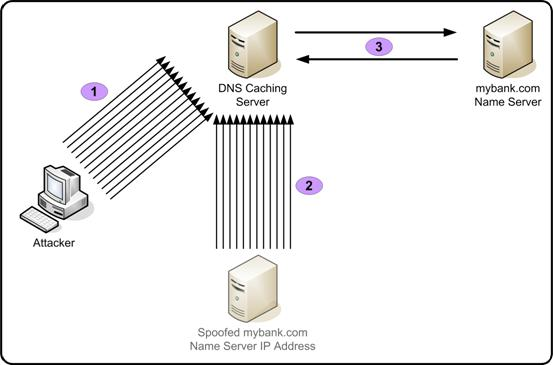
\includegraphics[width=\textwidth]{images/dns_spoofing_birthday.jpg}
	\caption{DNS Spoofing using multiple queries and Birthday Paradox \\ source : http://www.technicalinfo.net}
	\label{fig:DNSSpoofingBirthday}
\end{figure}

The attacker's aim is to trick the DNS cache server into thinking that the IP of www.mybank.com is the spoofed server's one, not the real one. This attack is used for phishing : as soon as the DNS cache server is compromised, users connecting to www.mybank.com will send their credentials to the attackers. \\
In order to do so, the attacker will send multiple queries : each DNS resolution is accompanied with a transaction ID which identify the query. The attacker's goal is to send resolution answers from this server with the correct transaction ID. The spoofed server send multiple resolution answers with random transaction ID. Since a DNS transaction ID is coded on 2 bytes, the pool of ID is no larger than 65535 : the birthday theorem stipulate that, with $n = 1.2 * \frac{\sqrt{65535}}{2}  = 153$  \footnote{ $n$ resolution queries$ + n$ answers $= 2*n$ total queries where looking for collision }queries, the attack has a 50\% chance of success\footnote{with 400 queries, the probability is over 99\%}. To further improve the probability of success, the attacker can also cripple the other server (the real one) with DDOS or bad routed packets in order to prevent him from sending a correct DNS resolution answer.

\section{Social Attacks}

Attacks target the weakest link of a system : sometimes it is the human nature the weakest link. This finding led to the famous "social engineering" attacks and the less known (but way more dangerous) rubberhose attacks.

\paragraph{Social Engineering}

Social Engineering describe a motley crew of methods designed to "punching a hole" into a system from the inside, without informing the insider of what he has done. \\
The most famous example is to leave some booby-trapped pendrives (and even more creative methods 
\footnote{ A mouse device with modified firmware was sent as a gift to tech-based company employees for a security test : \url{ http://www.theregister.co.uk/2011/06/27/mission_impossible_mouse_attack/}.  }
) on the company site and hope for one employee to plug it in his workstation . Once it is plugged, the rigged pendrive which usually contains a Trojan, execute its script in order to obtain a privilege escalation from within the system and connect to the attacker then.\\\\
A new type of Social Engineering has arisen with the emergence of social networks (Facebook, LinkedIn, ...) : in this type of attacks, the goal is to obtain a remote account of a target using infos about disseminated around the Web (email addresses, universities he has been, birthday, birth place, ...) and use it to gain access to his email account (using password reset and secret questions). Once the email account has been compromised, it can be used to launch phishing attacks on the real target and retrieve important secrets.


\paragraph{Rubberhose Cryptoanalysis}

The rubberhose attack describe the use of force (legal, hierarchical or physical) and/or torture on a physical person in order to extract information about the system (keys, ciphers used, ...). It is difficult to prevent those attacks since they are outside the scope of cryptanalysis (most of them belong to sociology/politics). The only way to mitigate against those attacks would be agent partial-blindness or plausible deniability.

\begin{figure}[hb!]
    \centering
       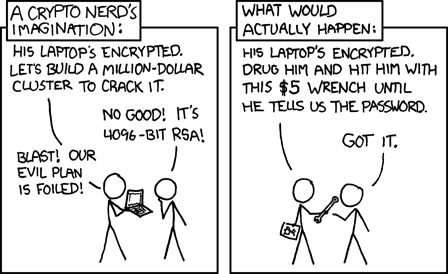
\includegraphics[width=0.7\textwidth]{images/rubberhose.png}
	\caption{Real-world 0-day exploit. \\ source : XKCD}
	\label{fig:RC4}
\end{figure}

\chapter{Standards Ciphers}


\section{One-Time Pad}

\subsection{XOR operator}

$\oplus$ : XOR operator (logic gate). Widely used in cryptography

\begin{table}[ht!]
	\centering
		\begin{tabular}{c|c|c}
			$A$ & $B$ & $A\xor B$ \\
			\hline
			0 & 0 & 0 \\
			0 & 1 & 1 \\
			1 & 0 & 1 \\
			1 & 1 & 0 \\
			\hline 
		\end{tabular}
	\caption{Table of logic for XOR}
	\label{tab:TableOfLogicForXOR}
\end{table}


\subsection{Cipher}
	$ E(k,m) = c = k \oplus m $ 
	$ D(k,c ) = m = k \oplus c$
	
	
\subsection{Vulnerabilities}

Facile a cracker une fois qu'on a un m et son c => k = m XOR c
Toutefois OTP a une perfect secrecy


\section{Data Encryption Standard (DES)}
\subsection{Feistel Network}
\subsection{DESx}

\chapter{Integrity}


This chapter will present the other aspect of cryptography : tampering prevention. An adversary can be able to do more than just eavesdropping : he can actually modify ciphertext messages on-the-go (using fro example a Man in the Middle attack). Therefore we need methods to ensure the non modification of the message during transmission.\\
In Dan Boneh's lecture, the integrity enforcement mechanisms are a minor part of the course, so this chapter will be quite succinct (especially since some generic constructions were already explained in the confidentiality chapter).


\section{Message Authentication Code (MAC)}

The most common way to enforce message integrity is to add a tag to the message, which will be verified upon reception. Moreover, the tag needs to be created using a secret key in order to prevent an attacker from fooling the verification algorithm.

\begin{mydef} $MAC = (S,V)$  
\begin{flushright}
	\begin{minipage}[t]{0.45\textwidth}
		\indent		 \textnormal{Tag Generator} \\
		\indent      $S: (k,m) -> t$   \\
	\end{minipage}
	\begin{minipage}[t]{0.45\textwidth}
		\indent	\textnormal{Verification Algorithm } \\
		\indent    $V: (k,m,t) -> {0,1}$ \\
	\end{minipage}
\end{flushright}
\end{mydef}

The tag and tag generation are more often called respectively ``hash'' and ``hashing''  : a hash function is an algorithm which takes variable-length data as input and outputs a fixed-length image of the input data. While being created in order to lessen the memory footprint of databases and speed-up the lookup of elements (hash tables, caches), hashing functions are also vastly used in cryptography. 
 
\subsection{Secure Mac}

The experiment needed to describe the security of a MAC mechanism is the same as for the cipher's semantic security : the attacker can submit 2 messages q times, and receive the tag of n ones. If it can't forge a new valid pair (m,t) to submit to V with a significant advantage, the MAC algorithm is considered secure.

\subsection{Collision Resistance}

The strength of a MAC against forged tags are closely related to the algorithm's resistance against collision attacks. A collision is a pair of messages $(m_0,m_1)$ such that $H(m_0) == H(m_1)$. We can clearly see that $m_0$ and $m_1$, if the MAC is using the hash functions $H$, have great chances to have the same tag. The verification algorithm will take one for another, which is a breach of security. \\
Therefore the algorithm for the tag generator has to be built upon collision resistant hashing functions.


\subsection{MAC Padding}
\label{sec:ISOPadding}

As for block ciphers, a hash algorithm works usually on a fixed length of plaintext information. However, contrary to the former, it is not possible to just pad the input text with 0's because it is insecure : the attacker can then send parts of the same message to retrieve important parts of information (block length, last digit digest ). \\
The standard (ISO) currently used is to pad with one $1$ and the rest with $0$'s.


\section{Constructions}

\subsection{Construction from PRF}

A secure MAC can be easily constructed from a PRF family. The following theorem is important since a lot of real-world MAC use it, in various environment (Internet, Banks, Defence, ..). 

\begin{mytheorem}[Secure MAC from PRF]
    If $F:K\times X \leftarrow Y$ is a secure PRF and $card(Y)$ is large, 
    then $I_F = (F, V_F)$ is a secure MAC and : 
   	%\begin{flushright}
\flushright	    $ Adv_{MAC} \leq Adv_{PRF} + \frac{1}{|Y|} $
	%\end{flushright}
\end{mytheorem}

The main interest of this theorem is we can produce fairly large hash function from concise pseudorandom function, as long as the output domain is large. The following paragraph will present well-known constructions to treat large input files.

\paragraph{CBC-MAC}



The CBC-MAC is constructed from a single PRP by cascading the output of the previous block into the current block's input. The last tag is pad with ??? and then hashed a final time with a different key. Finally, the last block is hashed by the same function but with a different key to produce the tag.

\begin{mytheorem}
	For every q-query adversary A attacking the CBC-MAC, there exist an adversary B attacking the PRP function F such that : 
	\begin{flushright}
 		$Adv_{PRP}[A,F_{ECBC}] = Adv_{PRP}[B, F] + 2\times \frac{q^2}{2.|K|}$	
	\end{flushright}
\end{mytheorem}

\begin{figure}[!ht]
	\centering
		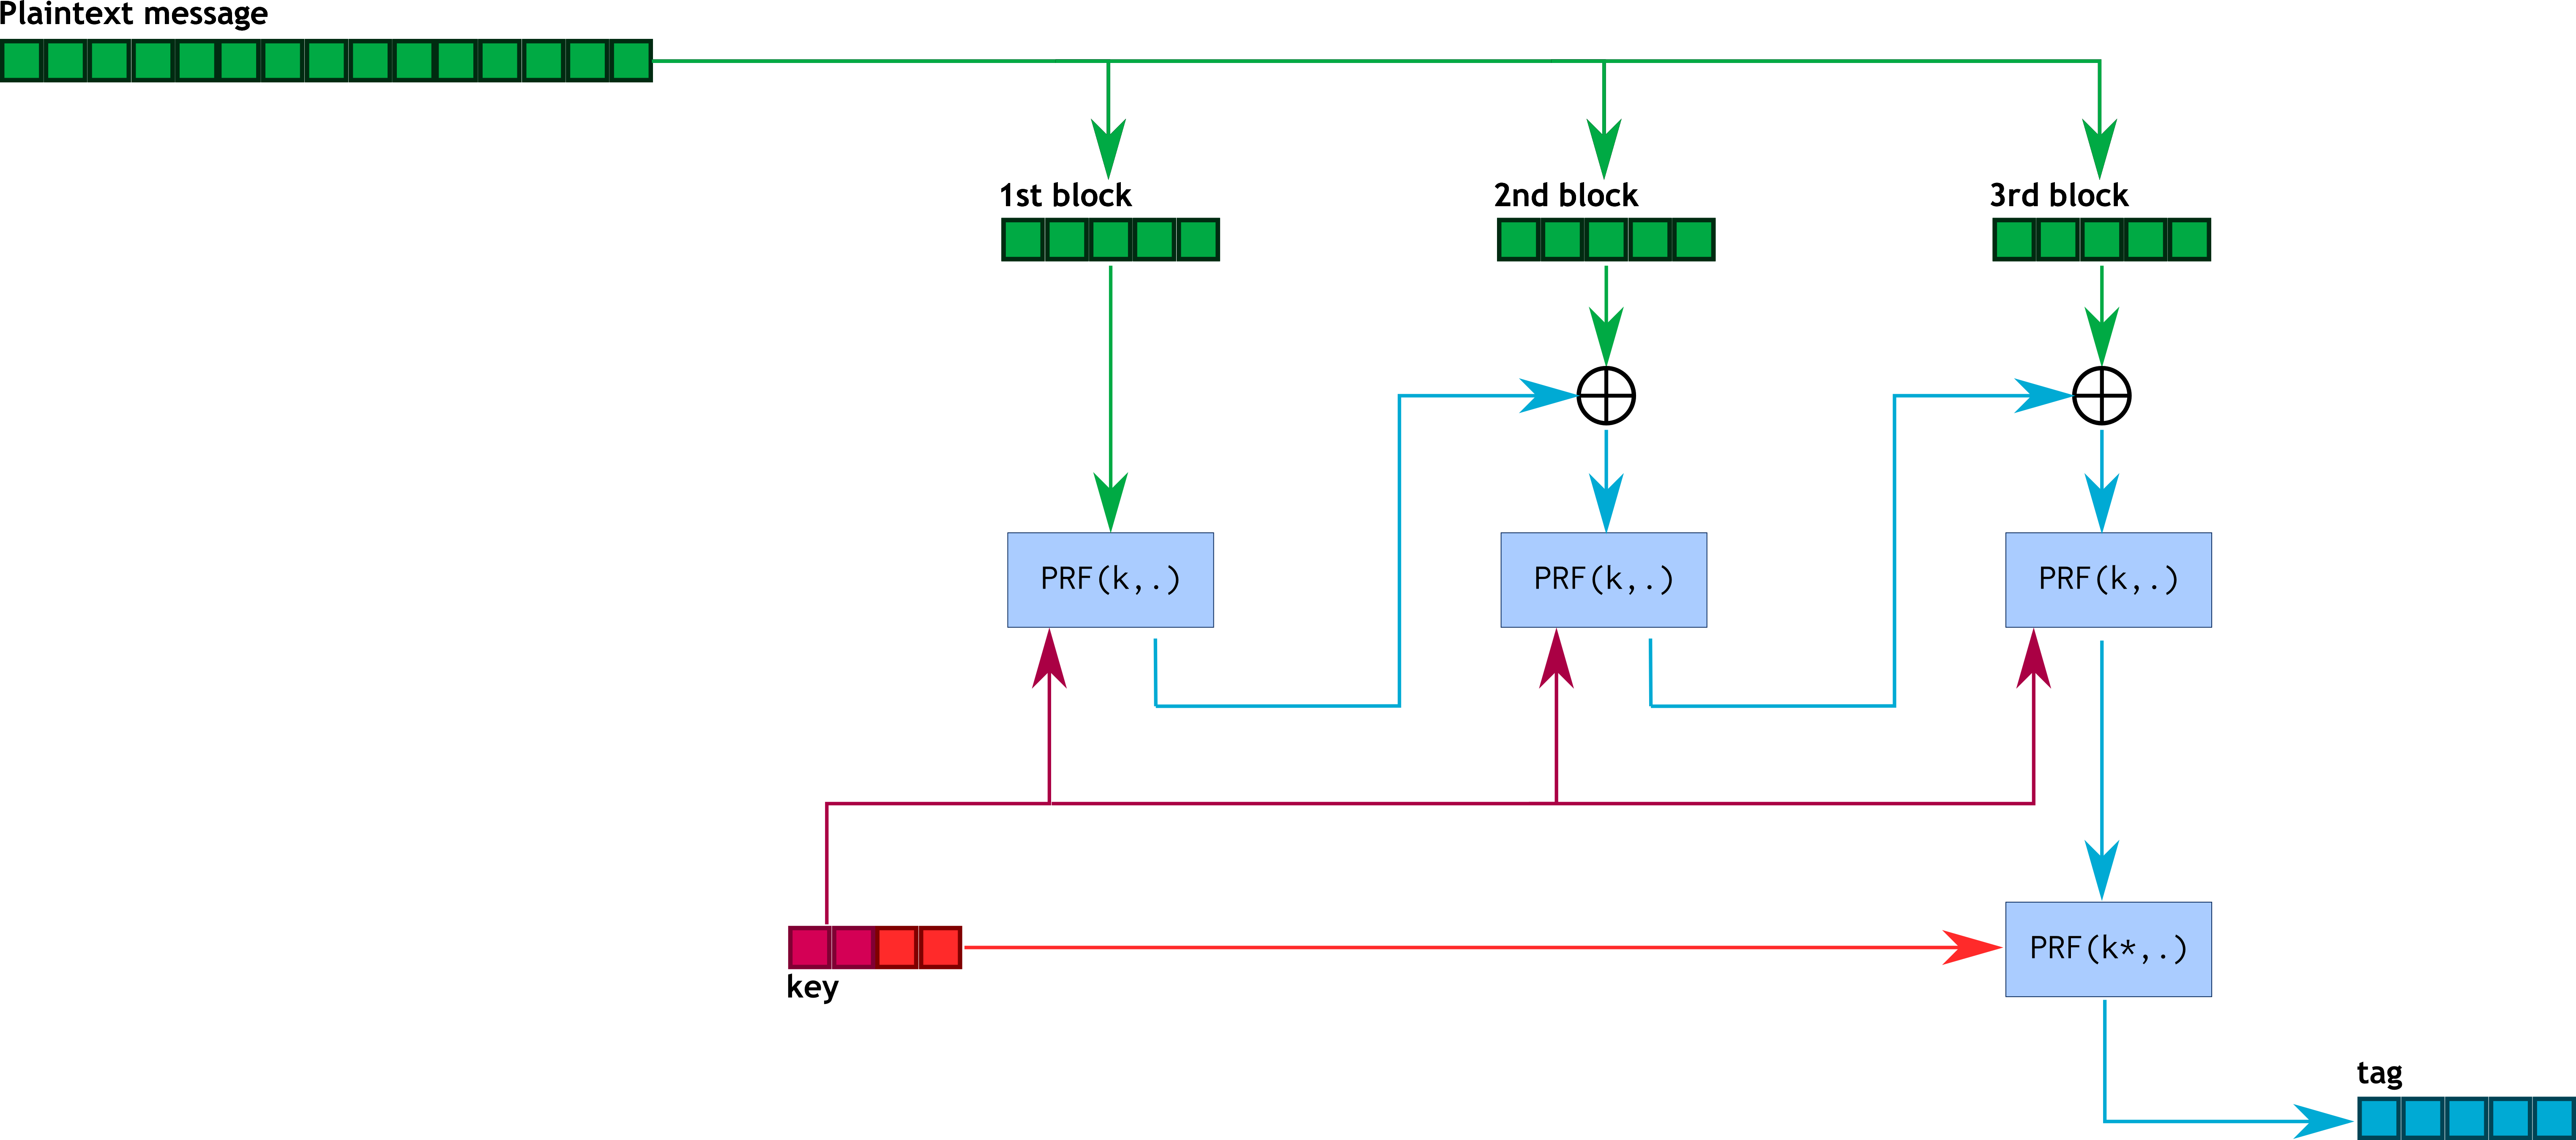
\includegraphics[width=0.7\textwidth]{CBC-MAC.PNG}
	\caption{CBC-MAC construction}
	\label{fig:CBCMACConstruction}
\end{figure}

\paragraph{NMAC}


In the NMAC construction, the output of a a block is used as the key for the next block. Like CBC-MAC, the process is fundamentally sequential.


\begin{mytheorem}
	For every q-query adversary A attacking the NMAC, there exist an adversary B attacking the PRF function F such that : 
	\begin{flushright}
 		$Adv_{PRF}[A,F_{NMAC}] = Adv_{PRF}[B, F] + 2\times \frac{q^2}{|X|}$	
	\end{flushright}
\end{mytheorem}

\begin{figure}[!ht]
	\centering
		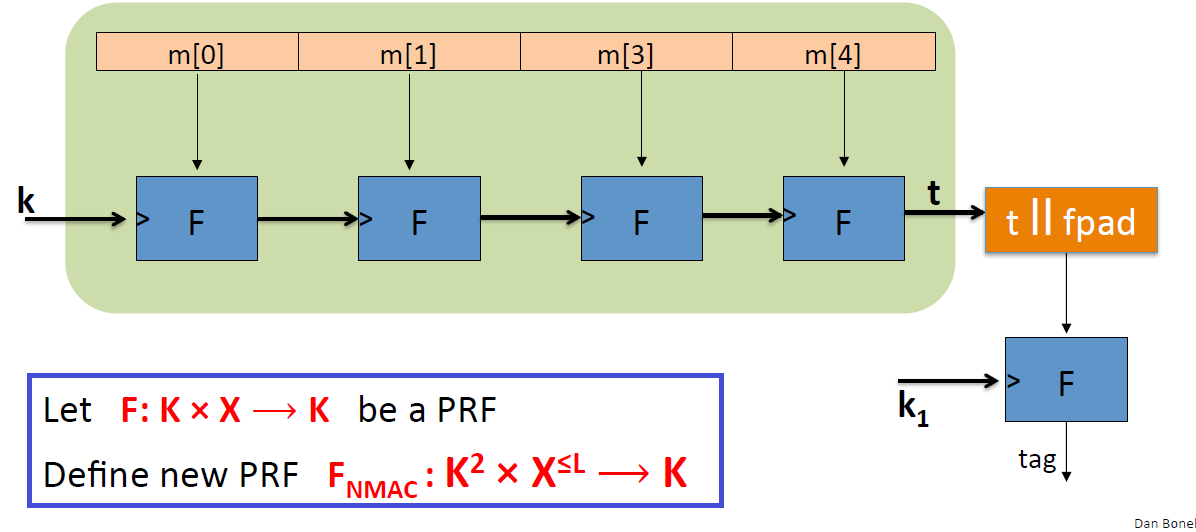
\includegraphics[width=0.7\textwidth]{NMAC.PNG}
	\caption{NMAC construction}
	\label{fig:NMACConstruction}
\end{figure}

\paragraph{PMAC}

The PMAC, or Parallel MAC, is obviously a parallel MAC construction : $P$ is a simple expansion function which will be used to fuzz the input data for each hash block. Like the previous constructions, the overall result is padded and hash one last time a second time to prevent oracle attack.

\begin{mytheorem}
	For every q-query adversary A attacking the PMAC, there exist an adversary B attacking the PRF function F such that : 
	\begin{flushright}
 		$Adv_{PRF}[A,F_{PMAC}] = Adv_{PRF}[B, F] + 2\times \frac{q^2\times L^2}{|X|}$	
	\end{flushright}
\end{mytheorem}

\begin{figure}[!ht]
	\centering
		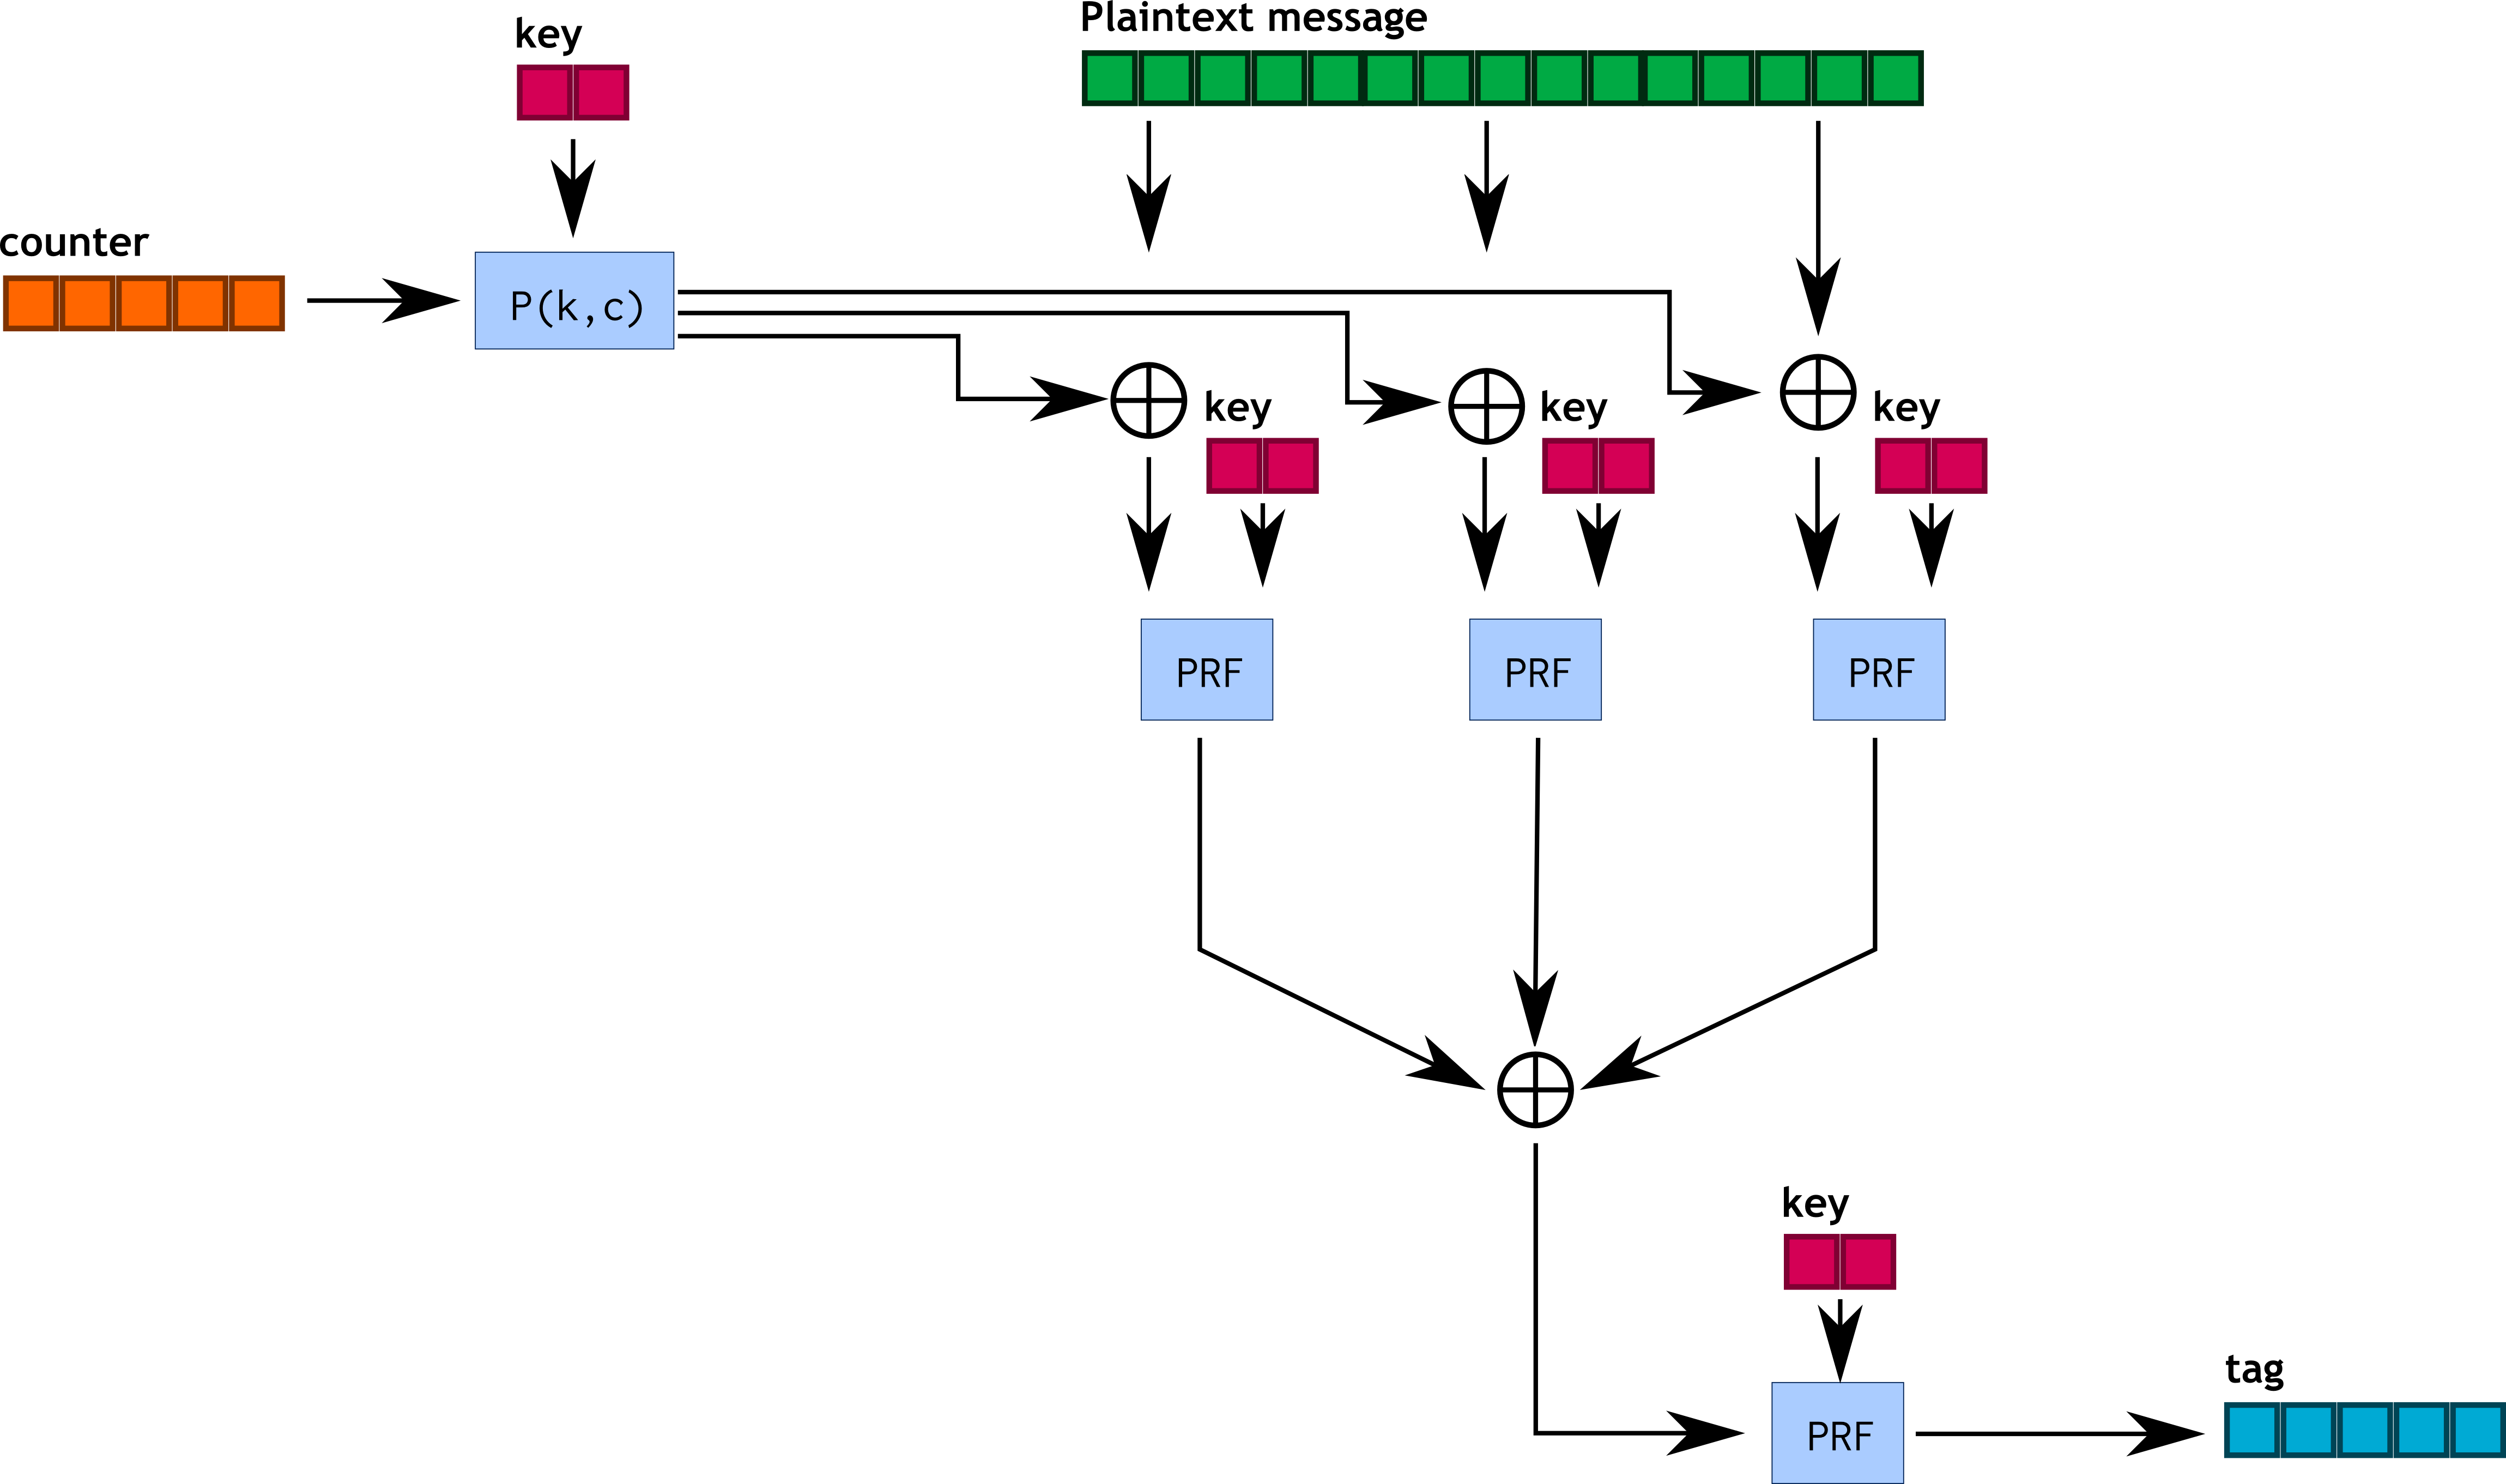
\includegraphics[width=0.7\textwidth]{PMAC.PNG}
	\caption{PMAC construction}
	\label{fig:PMACConstruction}
\end{figure}

\subsection{Construction from hash functions}

There is another method to construct secure MAC, from collision-resistant hash functions. A lot of famous MAC use this construction : SHA-1, SHA-2, etc.

\paragraph{Compression functions}

Compression functions are function that map two domains (let call them $M$ and $T$) with the following property : the output domain $M$ is several orders of size smaller than the input domain $T$ ($|M| \ll |T|$). Compression functions often take a fixed-size message and a key and output a fixed-sized message, which halves the overall message length. \\
Collision resistance is a fundamental property for compression functions used in secure MAC mechanisms. Others useful properties : easily computable, pre-image and second pre-image resistance. \\
Compression functions are often constructed from ciphers : for example the Davies-Meyer construction use a encryption cipher and some fuzzying steps to produce a collision-based hash function. This construction has the advantage of saving space, since the cipher can be used to encrypt and hash data (more on \ref{sec:AuthenticatedEncryption}).

\paragraph{Merkle-Damgard Paradigm}

The Merkle-Damgard architecture is a general layout to construct secure MAC mechanisms from collision-resistant hashing functions. It relies heavily on compression functions :

\begin{figure}[h!]
	\centering
		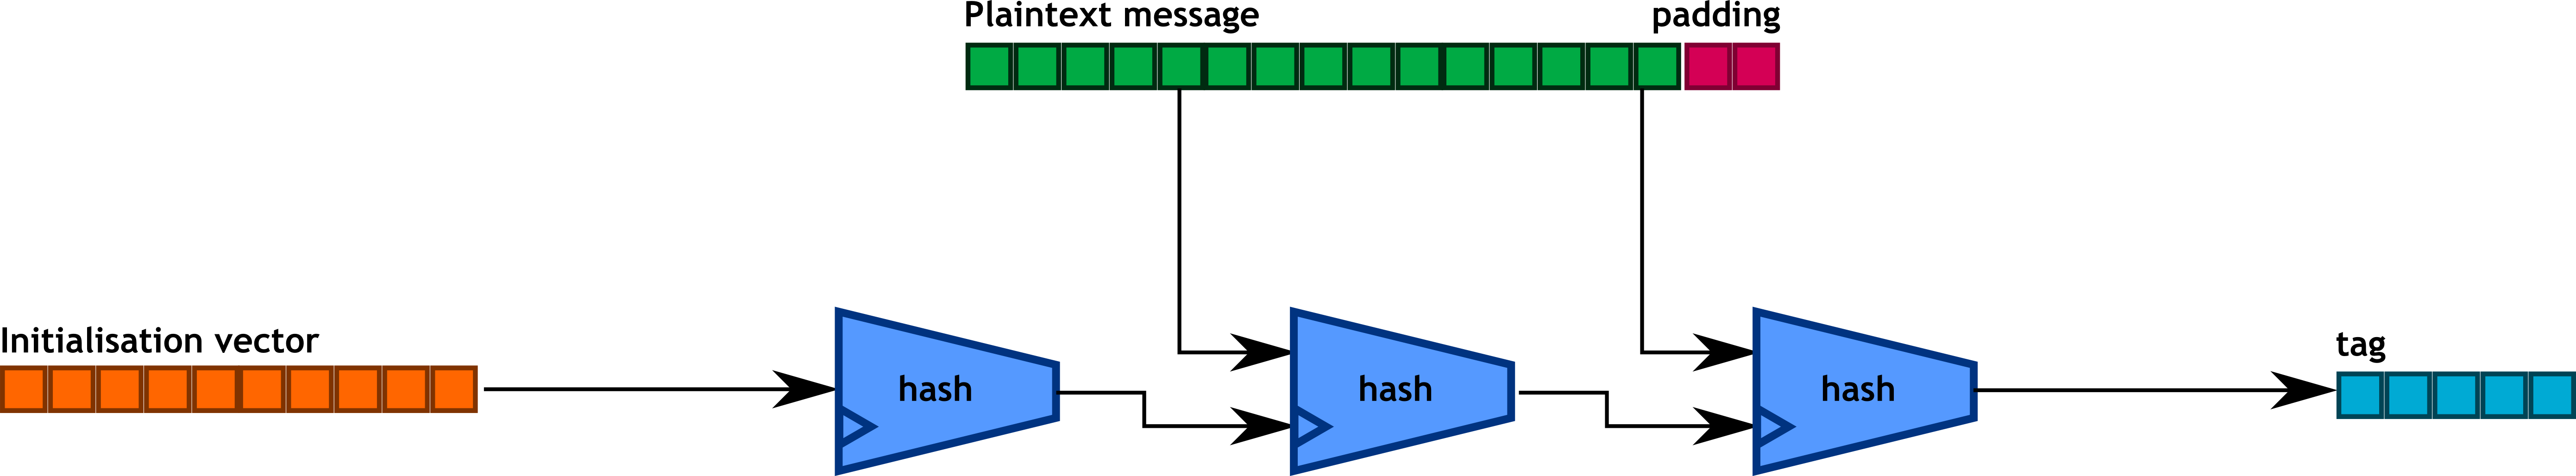
\includegraphics[width=0.7\textwidth]{Merkle-Damgard.PNG}
	\caption{Merkle-Damgard construction}
	\label{fig:MerkleDamgardConstruction}
\end{figure}

The construction is really similar to block ciphers : there is an initialization vector $IV$ to prevent replay attacks, several chained blocks of the same compression function, and a final padding. 

\paragraph{HMAC}

HMAC has two padding system : the inner pad $ipad$ and the outer pad $opad$.

\begin{figure}[h!]
	\centering
		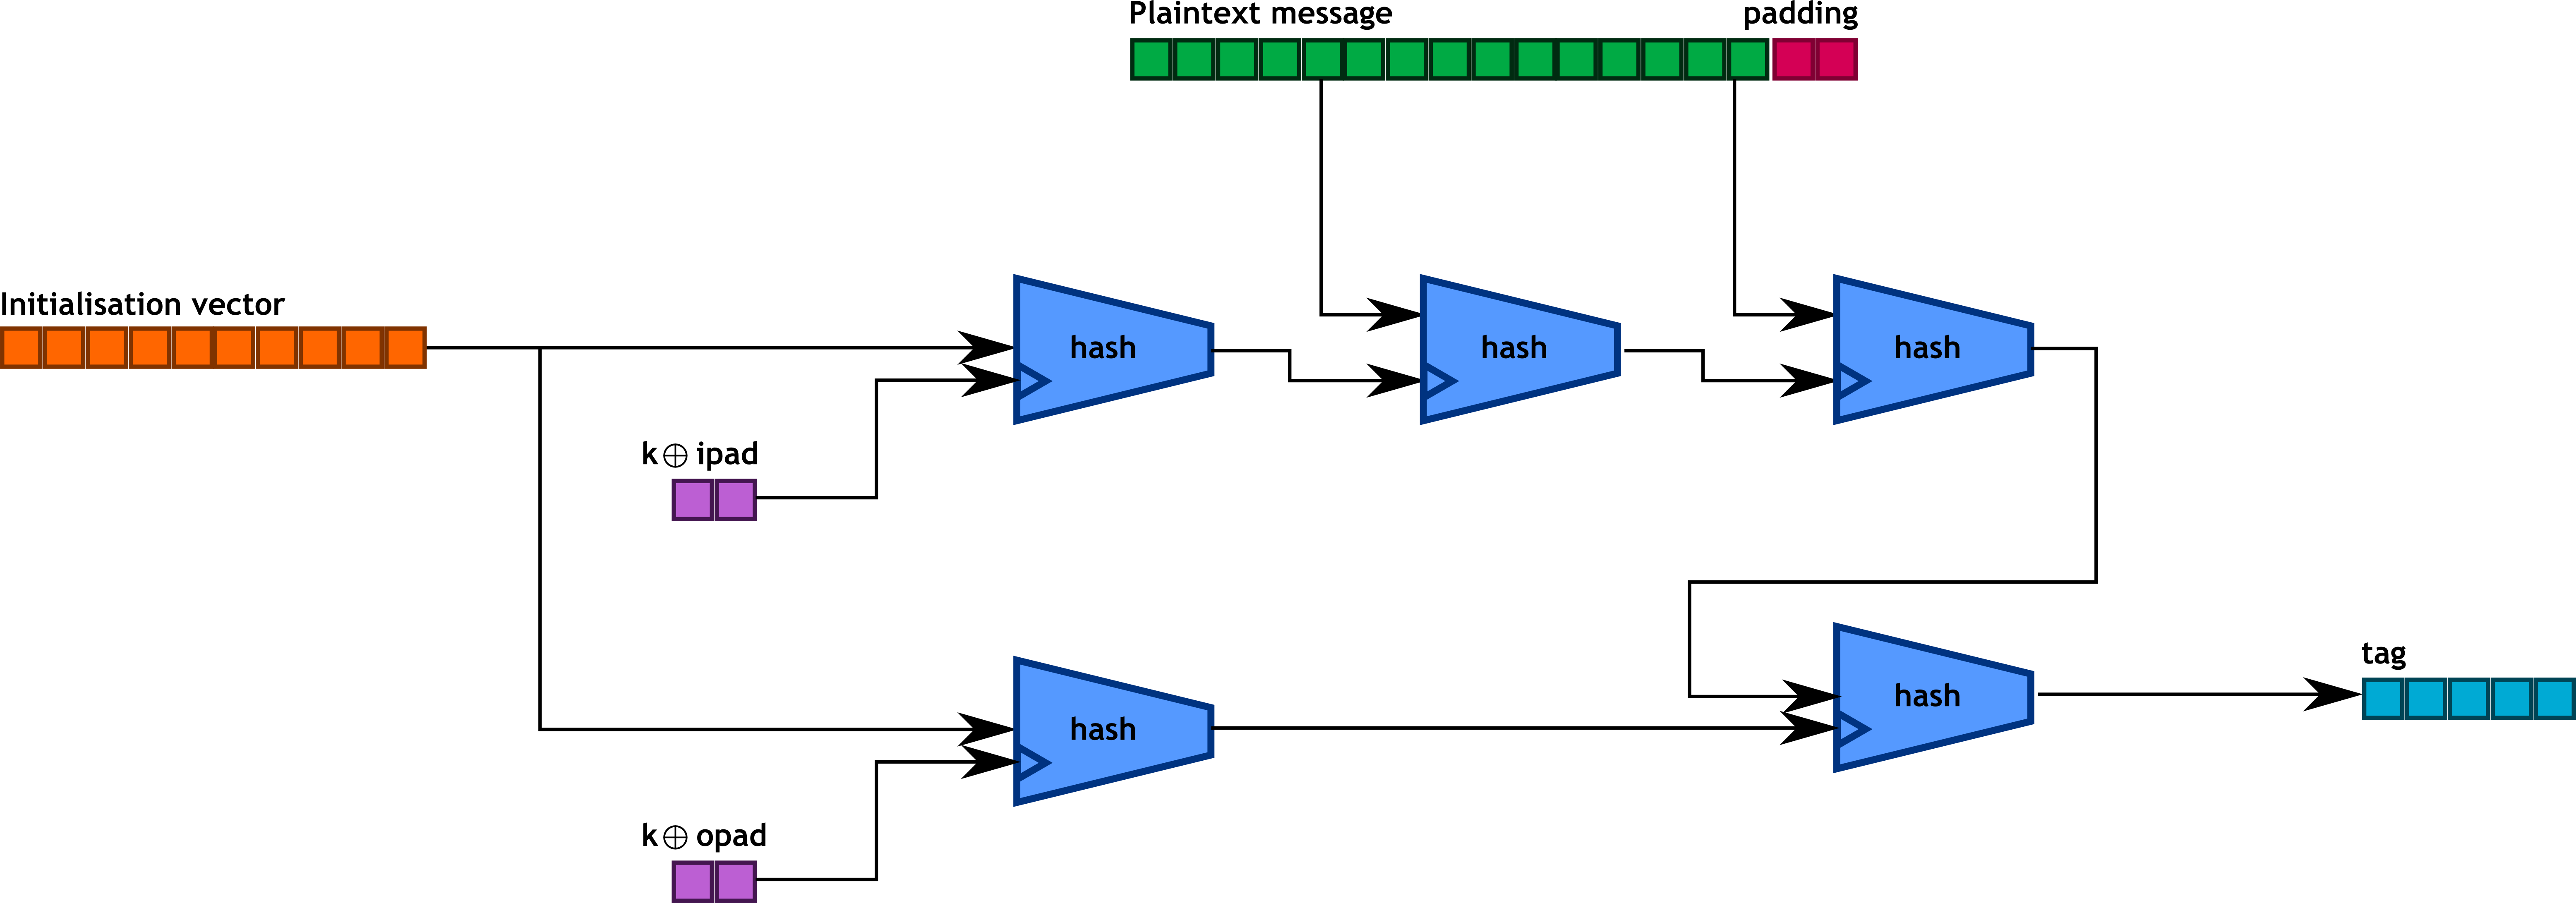
\includegraphics[width=0.7\textwidth]{HMAC.PNG}
	\caption{HMAC construction}
	\label{fig:HMACConstruction}
\end{figure}

\section{Authenticated Encryption}	
\label{sec:AuthenticatedEncryption}

Authenticated encryption is the following step in cryptography : ensuring integrity as well as confidentiality. In order to do that, it has to mix a MAC mechanism and a encrypting cipher. There is three approaches to the mixing :

\begin{description}
	\item[Encrypt-then-MAC :] This is the standard method, which yield the best results in terms of security.
	\item[Encrypt-and-MAC :]  Used for SSH.
	\item[MAC-then-Encrypt :] Used for SSL/TLS.
\end{description}


\subsection{Definition}

An authenticated encryption system consist of a cipher $(E,D)$ where : 
\begin{itemize}
	\item $E: KxM -> C$
	\item $D: KxC -> M\cup{\perp}$  ($\perp$ is the rejection symbol).
\end{itemize}

The system decrypt a ciphertext only if the MAC associated with has been validated. Otherwise, it will just output $\perp$. This symbol is important since it can prevent against oracle padding attacks : whether it's a invalid MAC or a pad error, the system has to output the same symbol in both cases.
\chapter{Key Exchange Protocols}

This chapter will focus on the communication aspect of cryptography, and more exactly on the initialisation part which contains the key-exchange protocols. As we seen in the last two chapters, it exists robust systems to ensure the confidentiality and integrity of data transitions against eavesdropping and active attackers (given that those systems were correctly implemented). However, these mechanisms does not describe how the two actors (generally called Alice and Bob) create a shared secret used to encrypt data. \\
Key-exchange protocol is the last part of Coursera Cryptography I class and it's more detailed in the second class.

\section{Trusted 3rd party}

The straight-up method of key-exchange between two parties (or more) is to use a third one as proxy. Each party gives their secret key to the TTP and, in return gives a shared one. While having many implementations (notary for wills and contract, Paypal for money transactions, certifications authorities (CA) ...) this procedure does not add security since it create a single point of failure (e.g. the TTP being pwn'ed) and the "trusted" part is sometimes false (as seen with the NSA leak ) : that's why it is preferable to look at zero-knowledge protocols for key exchange.


\section{Merkle Puzzles}
Merkle puzzles has been developed as a way to exchange keys using a generic symmetric cipher between two persons without a third-party. It's constructed upon a "puzzle", which means a computational difficult problem.\footnote{I will not try to define what is a "difficult" computational problem, look at NP-hard problems.} \\
As usual , we are in a situation of security against eavesdropping ( Merkle puzzles are insecure against active attacks such as AP poisoning ). Eve wants to retrieve the shared key that will be use for data transmission, and can only listen the communications between Alice and Bob. \\

Steps for key-exchange using Merkle puzzles :
\begin{enumerate}
	\item Alice prepares n problems, and send it to Bob. Each problem has a message encrypted containing an identifier and a secret key
	\item Bob solves one, and send the identifier in plaintext back to Alice
	\item Alice fetch the secret key corresponding to the identifier sent by Bob
	\item the two parties can communicate securely using their shared key.
\end{enumerate}

\paragraph{Complexity}

The strength of the Merkle puzzle scheme lies in the asymmetry of the problem. Let a Merkle Puzzle be of complexity linear $O(m)$.  Alice send n puzzles to Bob which solves one so Bob need $O(n+m)$ time computation. Bob sending back an identifier, Alice only need to solve one puzzle, thus $O(n+m)$ too. However, Eve needs to solve "all" (until the identifier is found) puzzles, so $O(n*m)$ : Alice and Bob needs linear time computation, while Eve needs quadratic time.\\

While being quite useful, the best gap in complexity provided by Merkle Puzzles is quadratic at best : for many real-world cases it is not enough\footnote{Merkle Puzzles are also vulnerable to quantum computation}. That's why exponential time gap scheme has been created (by Diffie and Hellman or RSA). 

\section{Diffie-Hellman protocol}
The Diffie-Hellman protocol is a key exchange scheme created in 1976, but still fairly used nowadays.  The strength of this protocol is based on the difficulty of the discrete logarithm problem. 

Steps : 
\begin{itemize}
	\item Alice and Bob choose a finite group (generally $\frac{\mathbb{Z}}{p\mathbb{Z}}$) and g a generator from this group. 
	\item Alice choose randomly a number $a$, and send to Bob $g^a$
	\item Bob does the same with $b$
	\item $g^{a.b}$ is the shared secret used to encrypt communications. Any eavesdropper has access to $g^{a}$ and $g^{b}$, but cannot easily compute the shared secret from these two numbers (since he has to compute either $a$ or $b$ using discrete log).
\end{itemize}

Discrete exponentiation is fairly easy ( linear time ) whereas discrete log is hard (best known algo in $exp(O(\sqrt[3]{x}))$ : this protocol use the asymmetry of the operation $\times $ to protect the key exchange, thus gaining the name of asymmetric-cryptography. However, if it were to be found an effective to the discrete log problem, the Diffie-Hellman would become insecure (as many others systems like El-Gamal).\\

This exchange is secure against eavesdropping, but not against Man-in-the-Middle attacks. The mitigation against it is to send, as well as $g^x$, a publicly certified signature from a trusted third party\footnote{More on digital signature in the second part of the Coursera course}.\\

\paragraph{Multi-party communication}
As seen previously the Diffie-Hellman protocol gives a secure way for two parties to exchange a secret. What about more than two people ? Unfortunately, this a currently an open problem \footnote{there is nonetheless a simple solution for 3 parties.} : there is no efficient way to create a multi-party shared secret.

\section{RSA encryption}


\subsection{Trapdoor Functions}

RSA encryption relies heavily on trapdoor functions for security. Trapdoor functions - or "one-way functions" - are easily computable in one direction, yet difficult in the other one \footnote{"easy" and "hard" does not have any formal meaning, we just look at difficulty from a empirical point-of-view}. \\

In cryptography, a trapdoor function is a triplet $(G, F, F_{-1})$ where :
\begin{itemize}
	\item $G$: $ seed \rightarrow (pk, sk) $ a randomized algorithm which produce a public key and a secret one.
	\item $F$ : $ (pk, X) \rightarrow  Y $ used to encrypt message $X$ using public key $pk$.
	\item $F_{-1}$ : $ (sk, Y) \rightarrow X $ used to decrypt ciphertext $Y$ using secret key $sk$.
\end{itemize}

\begin{mytheorem}
	$\forall (pk,sk) $ generated by $G$, \\
	$\forall m \in M $, $F_{-1}( sk, F(pk, m) ) = m $
\end{mytheorem}

\subsection{RSA Trapdoor}

The RSA trapdoor function relies on the prime factorization problem and the modular e-roots' problem. \\
First, the prime factorization problem : given two prime numbers, it's easy to compute their product. However, given the product of two primes numbers, it is fairly difficult to find the factorization. That's mean we can communicate the primes' product publicly without lessening the security of the protocol - the two primes still has to be big enough -. In the case of RSA, the primes' product number will be used as a generator for (Z/nZ).\\
Secondly, the modular e-roots' problem : given a number and an exponent, it is easy to compute its exponentiation in Z/nZ, but it is difficult to compute the e-root in the same group (in the math sense).


\section{Public Key Encryption}

% 3 tools : 
% Asymmetric encryption for key-exchange : ( G, F, F-1 )
% Symmetric encryption for communication : (E, D)
% Hash function for integrity			 :  H

% Encryption :
% G() -> (pk, sk)

% x is chosen randomly
% E(pk, m) ->  |F(pk,x)||Es( H(x), m )|





\section{El Gamal}







>>>>>>> Trusted authorities and Diffie-Hellman
>>>>>>> refs/remotes/palin/master

\chapter{Miscellaneous}

In this chapter, we will cover various minor parts of cryptography which does not belong to the previous chapters, e.g. stenography, key derivation, deterministic encryption, ...

\section{Stenography}
% "Hide in plain sight"

\section{Key derivation}

\section{Deterministic Encryption}


\section{Arithmetic Algorithms}

In this section, we will discuss big integer manipulation. Most computer have 32/64-bit architecture, while cryptography typically handle hundreds-bits number : the operations like addition or multiplication are not atomic.

basic operations :
addition -> linear time
multiplication -> $O(n^(2))$ up to $O(n.log(n))$(asymptote). currently best : $O(n^{1.585})$.
division with remainder -> $O(n^(2))$


exponentiation in $Z_N$ -> $O( Multi*log(n) )$ <= $O(n^2.log(n) )


%%%%%%%%%%%%%%
%% Summary

%%%%%%%%%%%%%%
%% Cites


\end{document}
%%%%%%%%%%%%%%%%%%%%%%%%%%%%%%%%%%%%%%%%%%%%%%%%%%%%%%%%%%%%%%%%
%% 
%%%%%%%%%%%%%%%%%%%%%%%%%%%%%%%%%%%%%%%%%%%%%%%%%%%%%%%%%%%%%%%%